\subsubsection{Rondell System}

Eine der zwei vorgestellten Varianten basiert teilweise auf dem Rondell-Modell der Konkurrenz, jedoch mit dem Unterschied, dass die Fahrräder von außen, anstatt von innen ausgelagert werden. Zudem werden die Fahrräder nicht auf Schienen, sondern in Boxen gelagert, welche dann zusammen ein und ausgelagert werden. Die abgeschlossenen Boxen verringern zwar die Platzeffizienz, jedoch sind sie sicherer und erlauben höheren Zusatznutzen. Das System ist hinsichtlich der ringförmigen Anordnung der Fahrräder sehr ähnlich wie bestehende Varianten. Je nach Bedarf können unterschiedlich viele Ebenen übereinandergestapelt werden.

\begin{figure}[H]
  \centering
  \begin{subfigure}{0.39\textwidth}
    \centering
    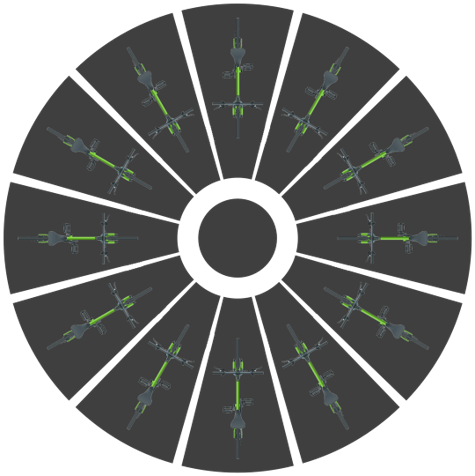
\includegraphics[width=\textwidth]{images/rondell_skizze_oben.png}
    \caption{Ringförmige Anordnung der Fahrräder}
    \label{fig:rondell_skizze_oben}
  \end{subfigure}
  \begin{subfigure}{0.39\textwidth}
    \centering
    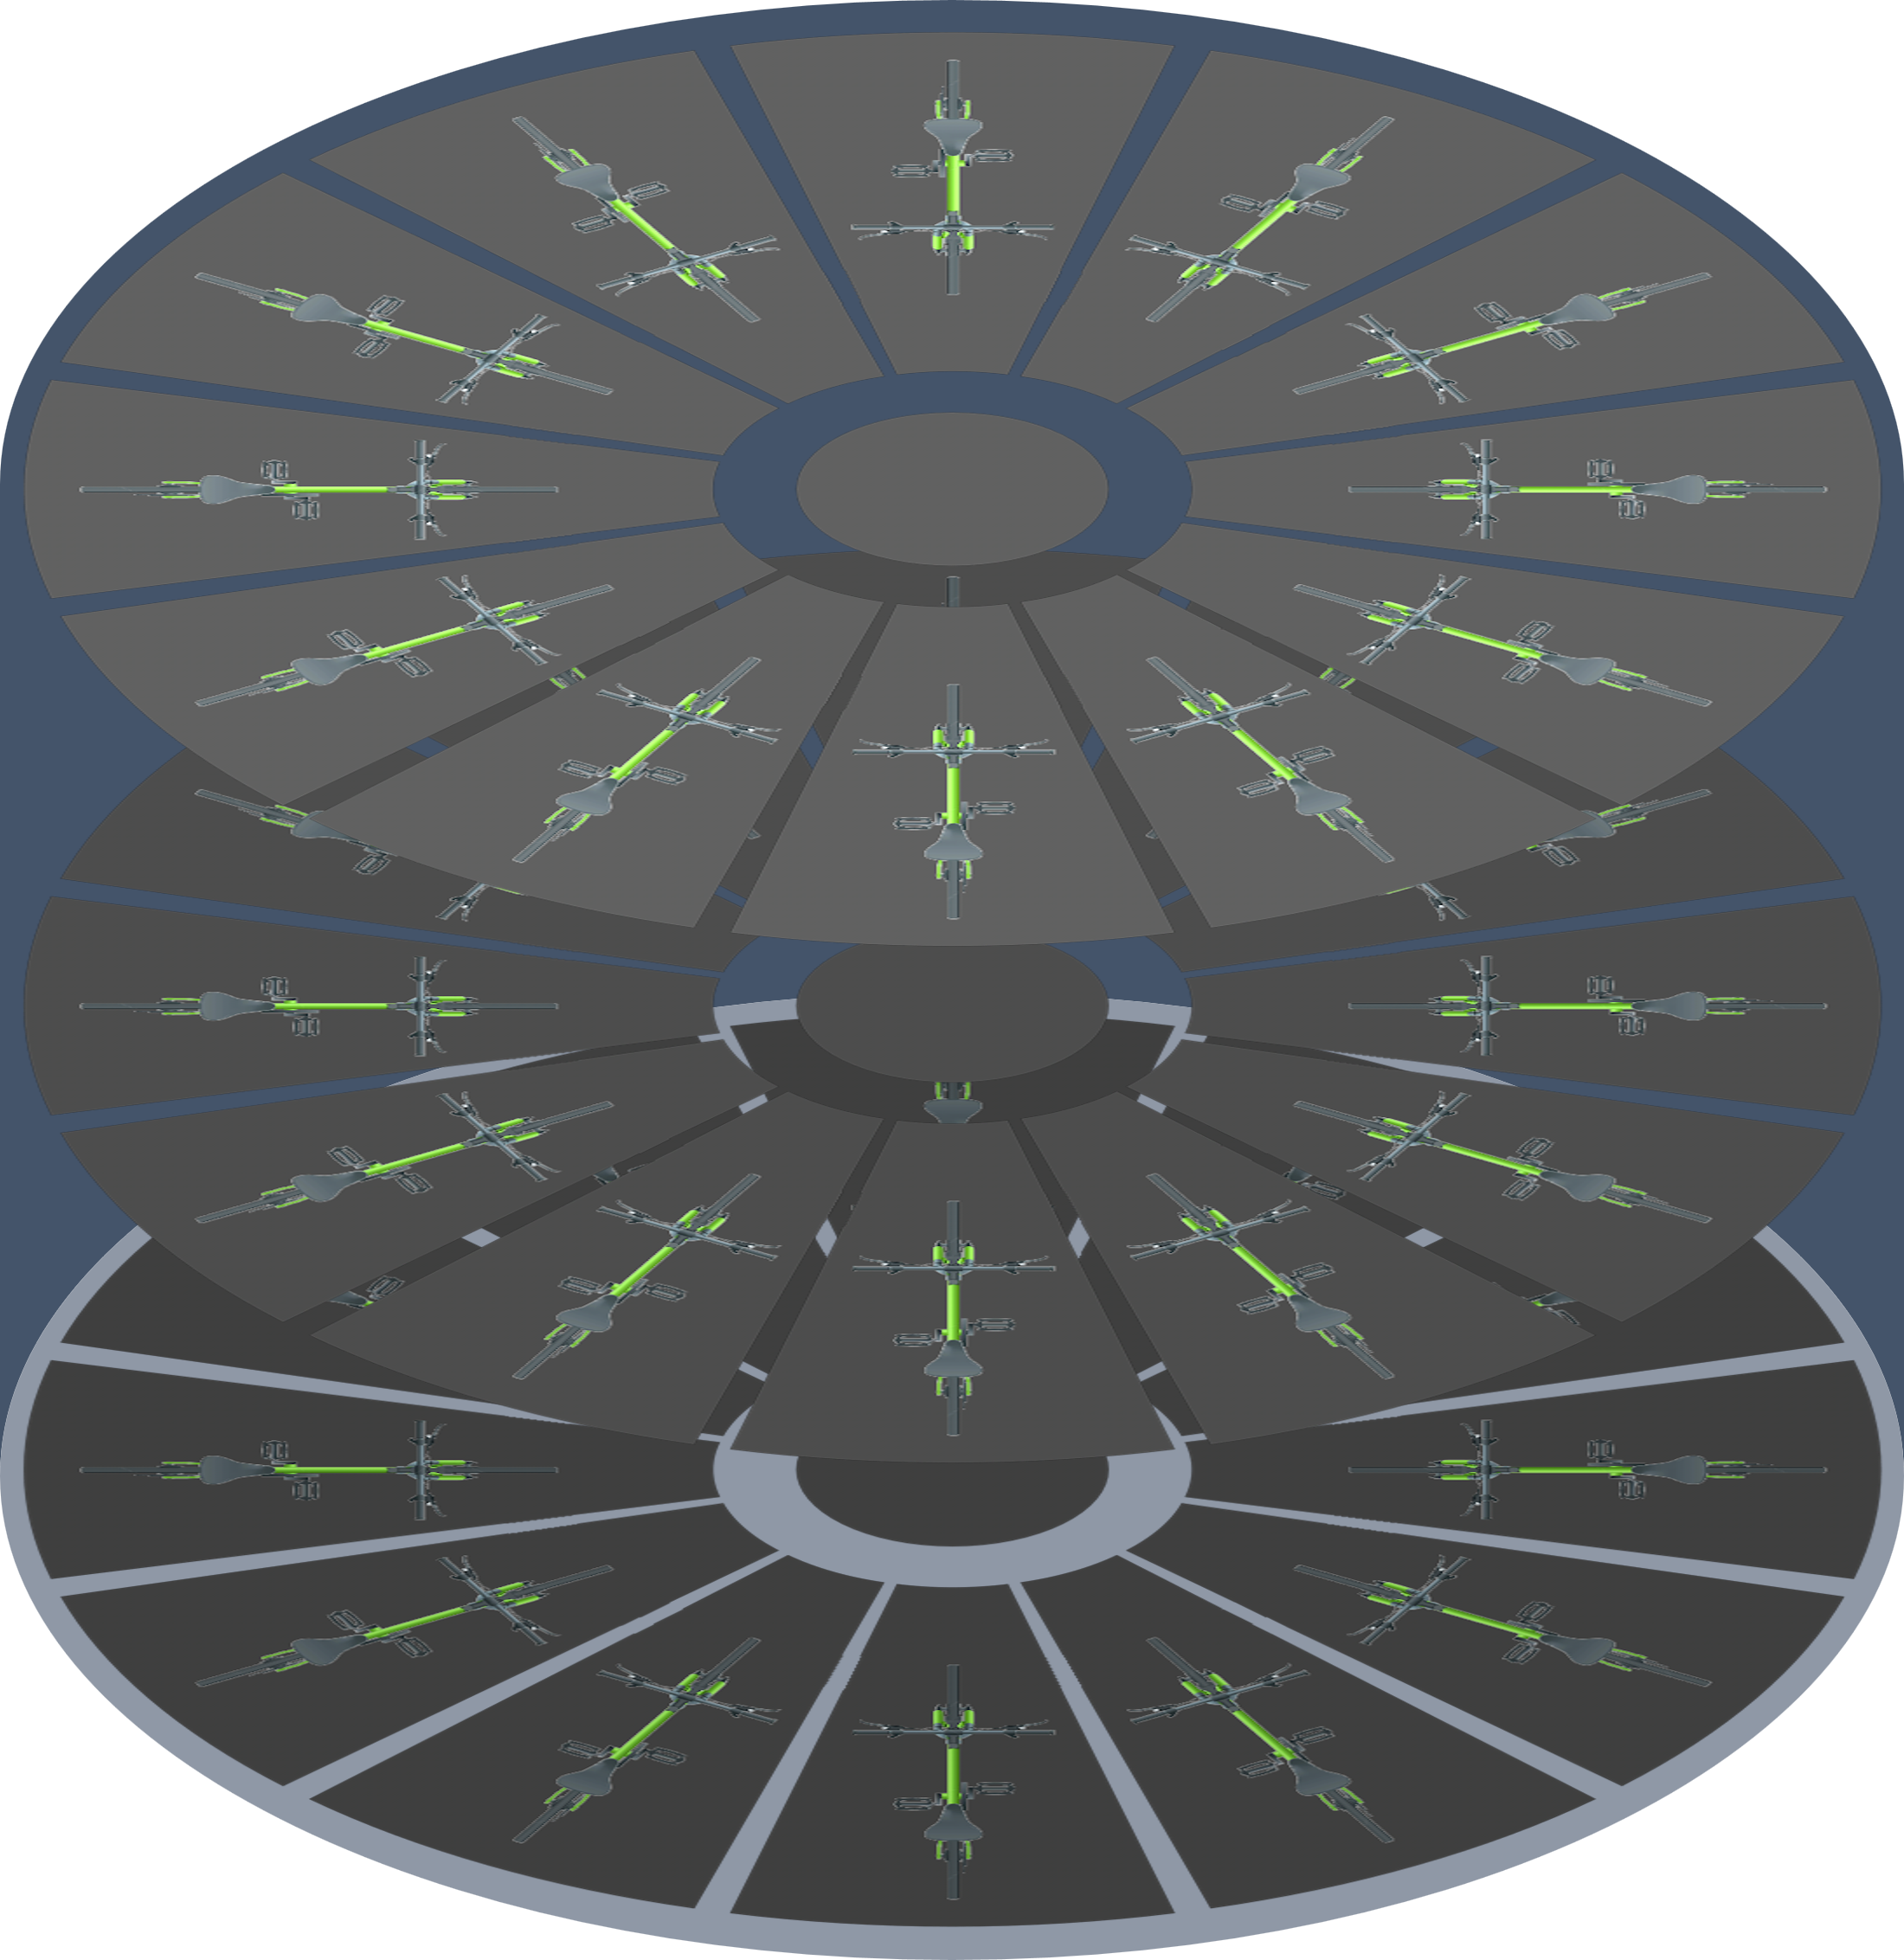
\includegraphics[width=\textwidth]{images/rondell_skizze_seite.png}
    \caption{Ringförmige Anordnung der Fahrräder auf mehreren Ebenen}
    \label{fig:rondell_skizze_seite}
  \end{subfigure}
\end{figure}

\clearpage
\paragraph{Auslagerung} Bei einer ringförmigen Formation an Lagerplätzen bieten sich zwei Möglichkeiten an, Fahrräder zu entnehmen:

\subparagraph{Auslagerung von innen} Bei der Auslagerung von innen werden die Fahrräder mittels eines in der Mitte gelegenen Lagerroboter aus- und eingelagert. Herkömmliche Fahrradlagersysteme verwenden diese Variante. Dieses System hat den Vorteil, dass mit einem einzelnen Lagerroboter alle Fahrräder bewegt werden können. Gleichzeitig bedeutet dies aber auch, dass dieser Roboter alle Fahrräder bewegen muss, was zu Staus führen kann. Ein weiterer Nachteil ist, dass durch die vorliegende Geometrie eines solchen Systems viel Platz verschwendet wird. Dies ist vor allem der Fall, wenn die Fahrräder in Boxen gelagert Werten

\begin{figure}[H]
  \centering
  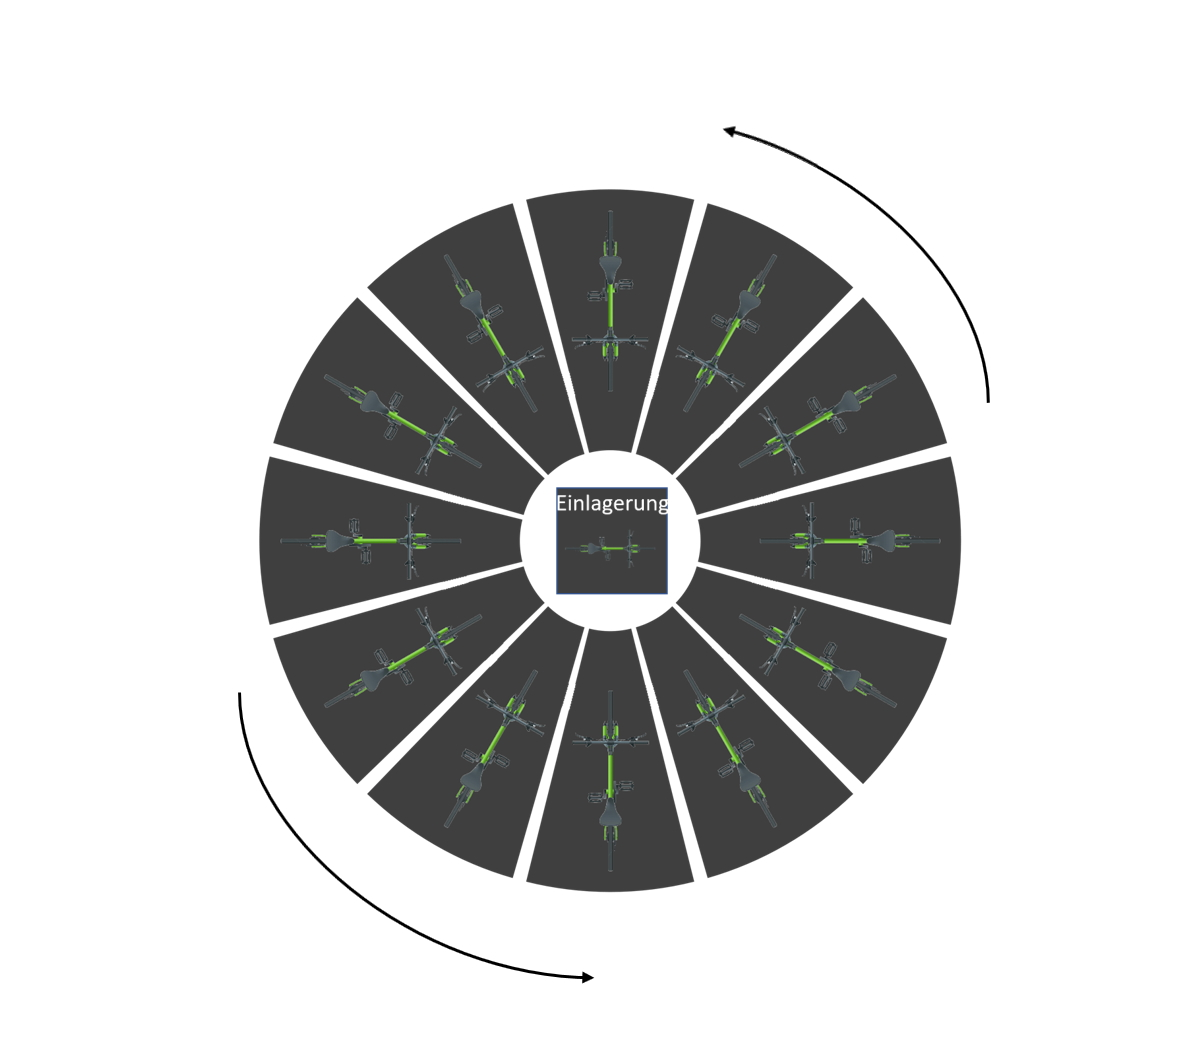
\includegraphics[width=0.3\textwidth]{images/rondell_innen.jpg}
  \caption{Rondell System mit Auslagerung von innen}
  \label{fig:rondell_innen}
\end{figure}

\subparagraph{Auslagerung von außen} Bei der Auslagerung von außen werden die Fahrräder mittels eines Lifts von außen manipuliert. Im Gegensatz zur Auslagerung von innen drehen sich hier die einzelnen Ebenen und nicht der Lagerroboter selbst. Je nach Bedarf kann die Anzahl der Lagerroboter angepasst werden und optimal auf die Anforderungen des Standorts zugeschnitten werden.

\begin{figure}[H]
  \centering
  \includegraphics[width=0.3\textwidth]{images/rondell_außen.jpg}
  \caption{Rondell System mit Auslagerung von außen}
  \label{fig:rondell_außen}
\end{figure}

\clearpage
\paragraph{Mögliche Umsetzung} Das System erlaubt große Flexibilität hinsichtlich Umsetzung und kann falls benötigt auch modular erweitert oder verkleinert werden. Parameter, welche je nach Anwendung geändert werden könnten, beinhalten Anzahl an Fahrrädern pro Ebene, Anzahl an Ebenen und Anzahl an Einlagerungsliften. Ein Beispiel für eine solche Variante ist auf der folgenden Abbildung zu sehen.

\begin{figure}[H]
  \centering
  \begin{subfigure}{0.49\textwidth}
    \centering
    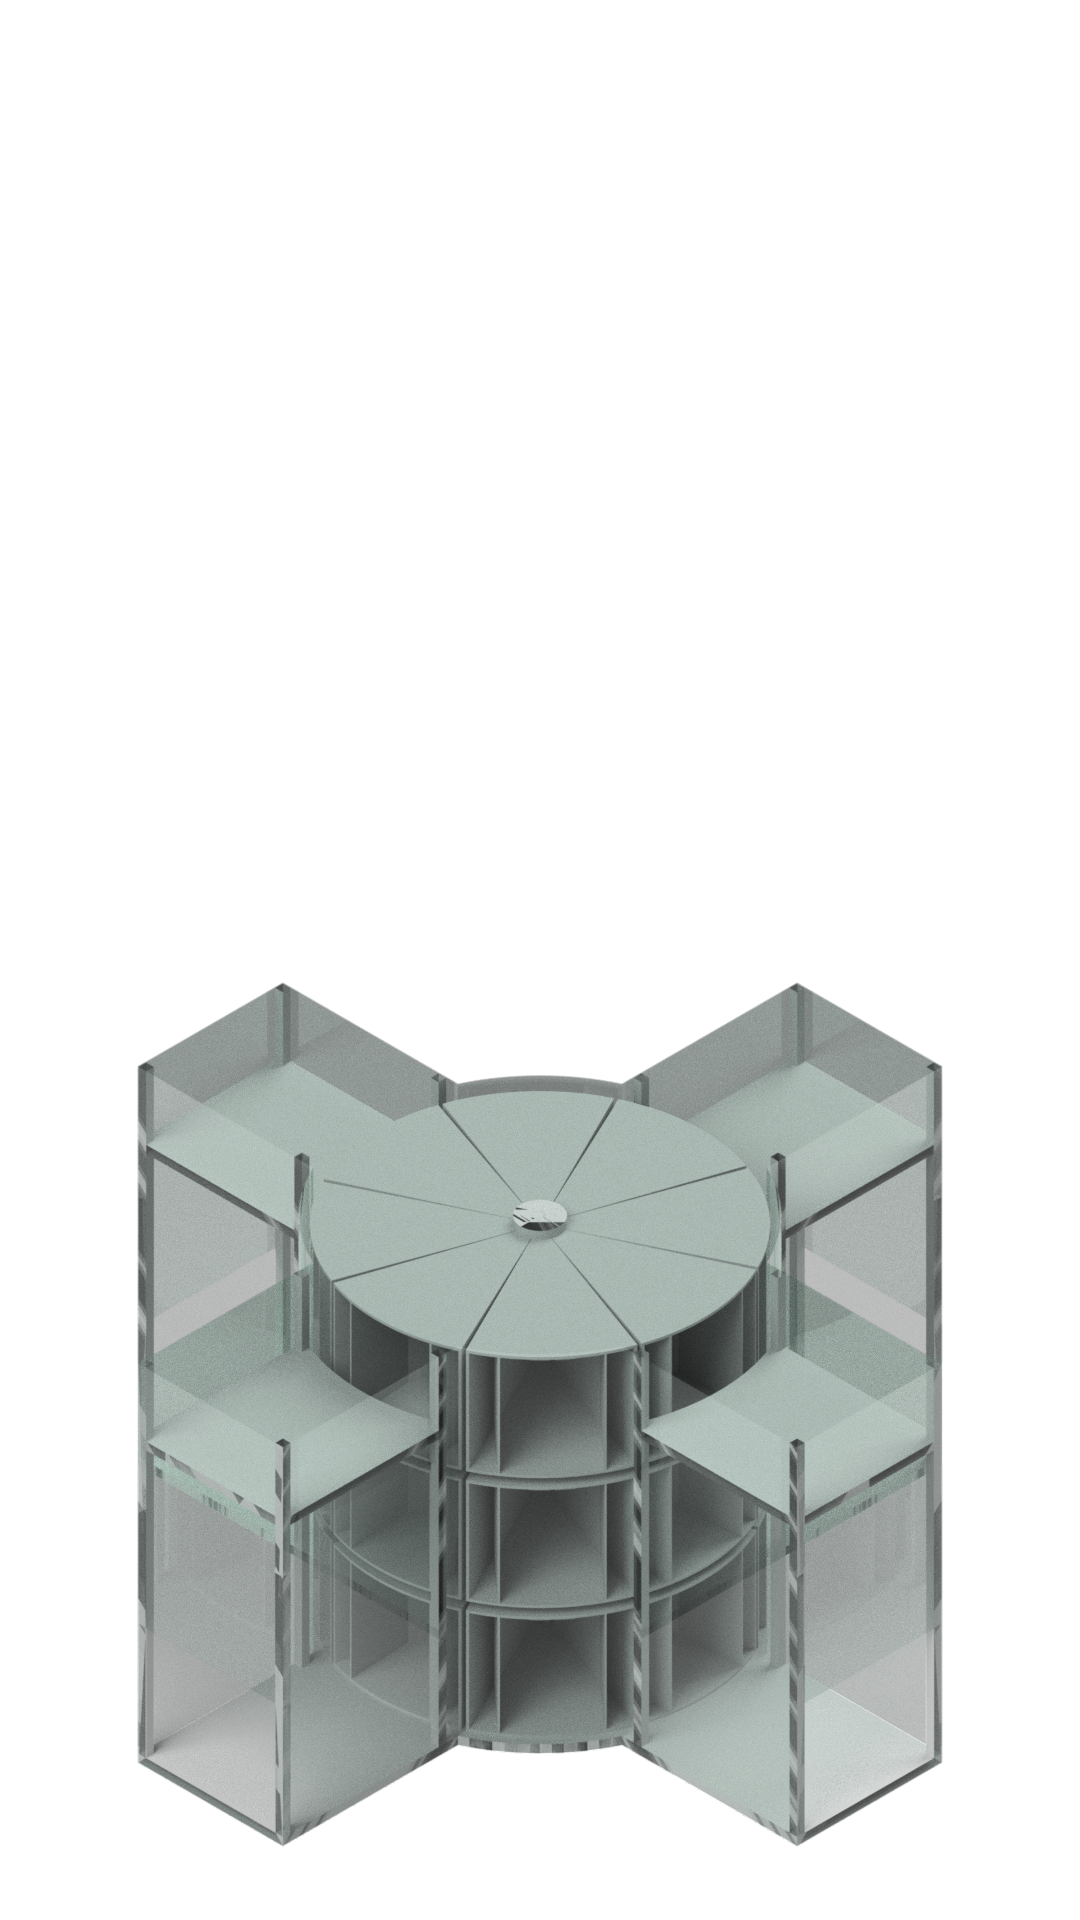
\includegraphics[width=\textwidth]{images/rondell_3.png}
    \caption{Rondell System mit 3 Ebenen}
    \label{fig:rondell_3}
  \end{subfigure}
  \begin{subfigure}{0.49\textwidth}
    \centering
    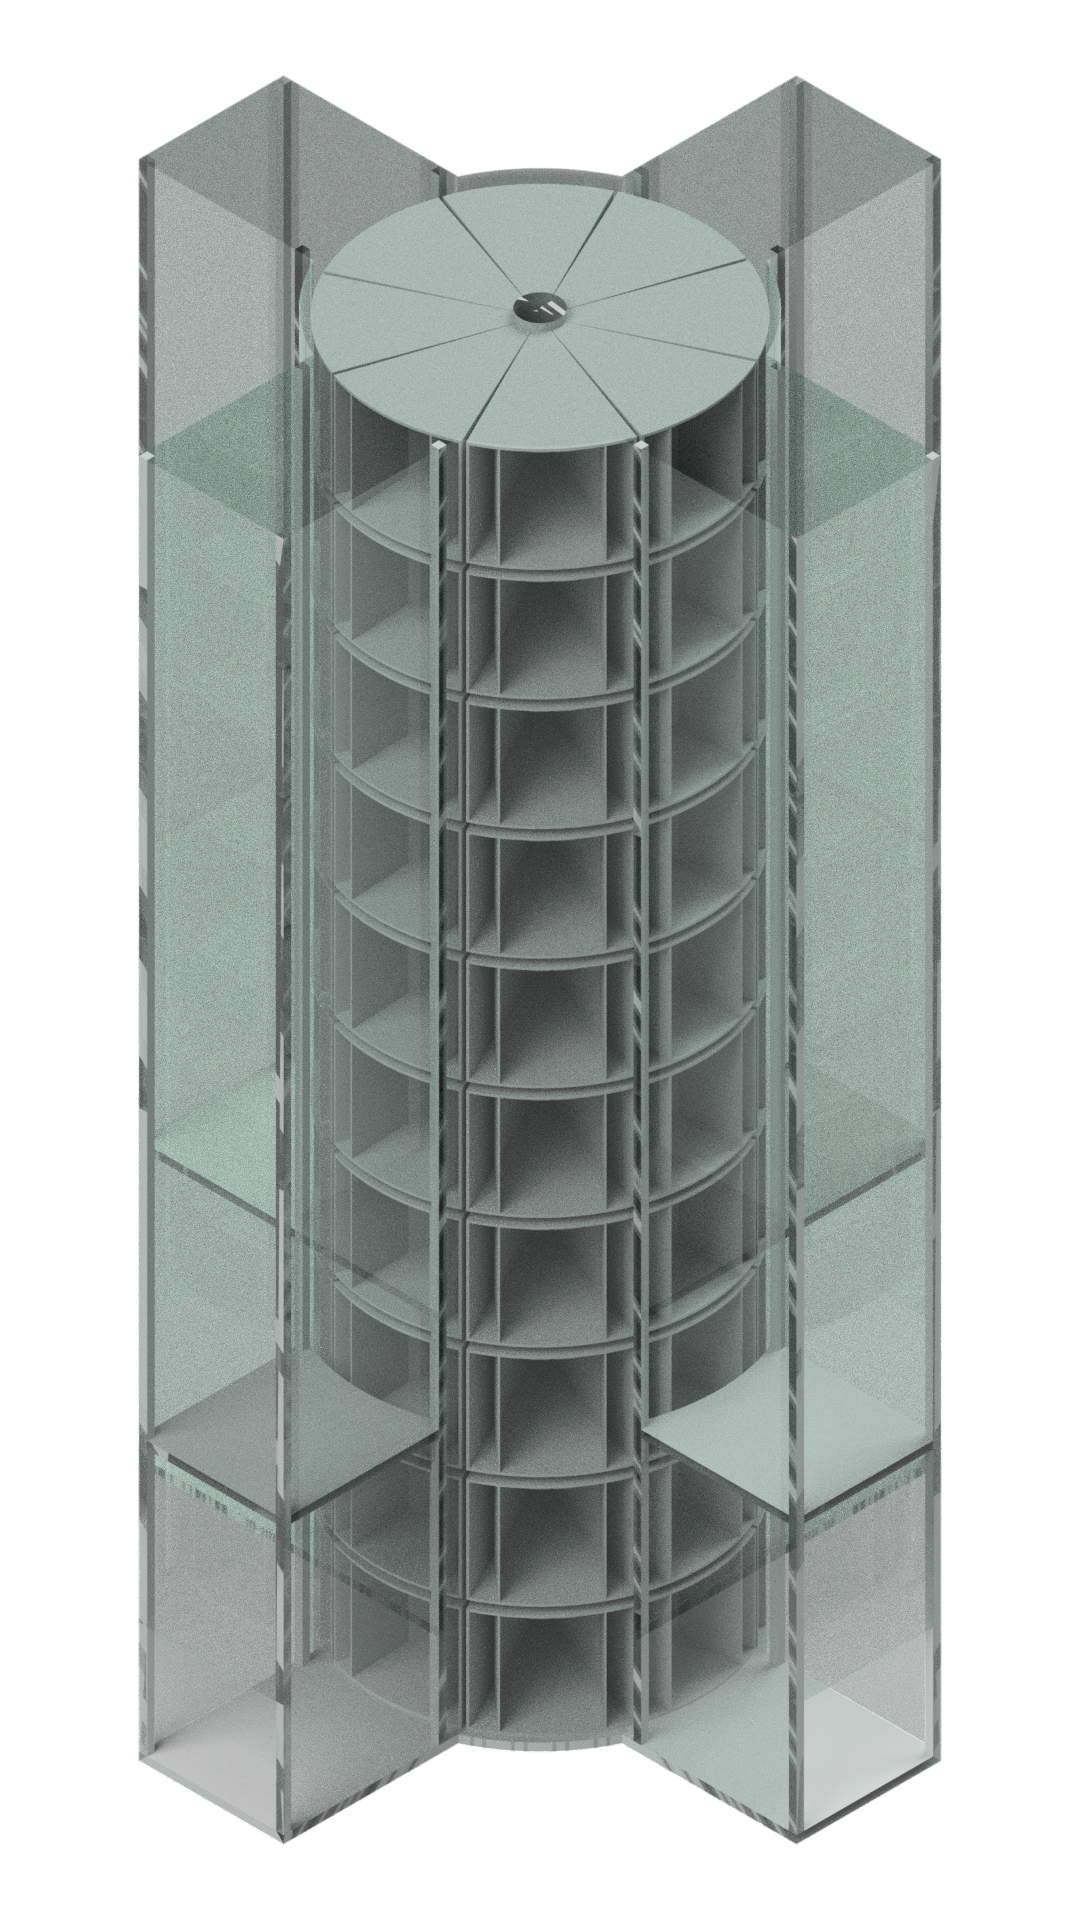
\includegraphics[width=\textwidth]{images/rondell_10.png}
    \caption{Rondell System mit 10 Ebenen}
    \label{fig:rondell_10}
  \end{subfigure}
\end{figure}

\clearpage
\paragraph{Konstruktionsgetriebene Analysen} Um den optimalen Platzverbrauch zu garantieren, wurde die technische Zeichnung mit verschiedenen Parametergrößen untersucht. Eine dieser Größen ist der Durchmesser des „Rückgrats“ des Turms, in dem die ganze Technik verbaut ist und an der die Ebenen gelagert werden.

\begin{figure}[H]
  \centering
  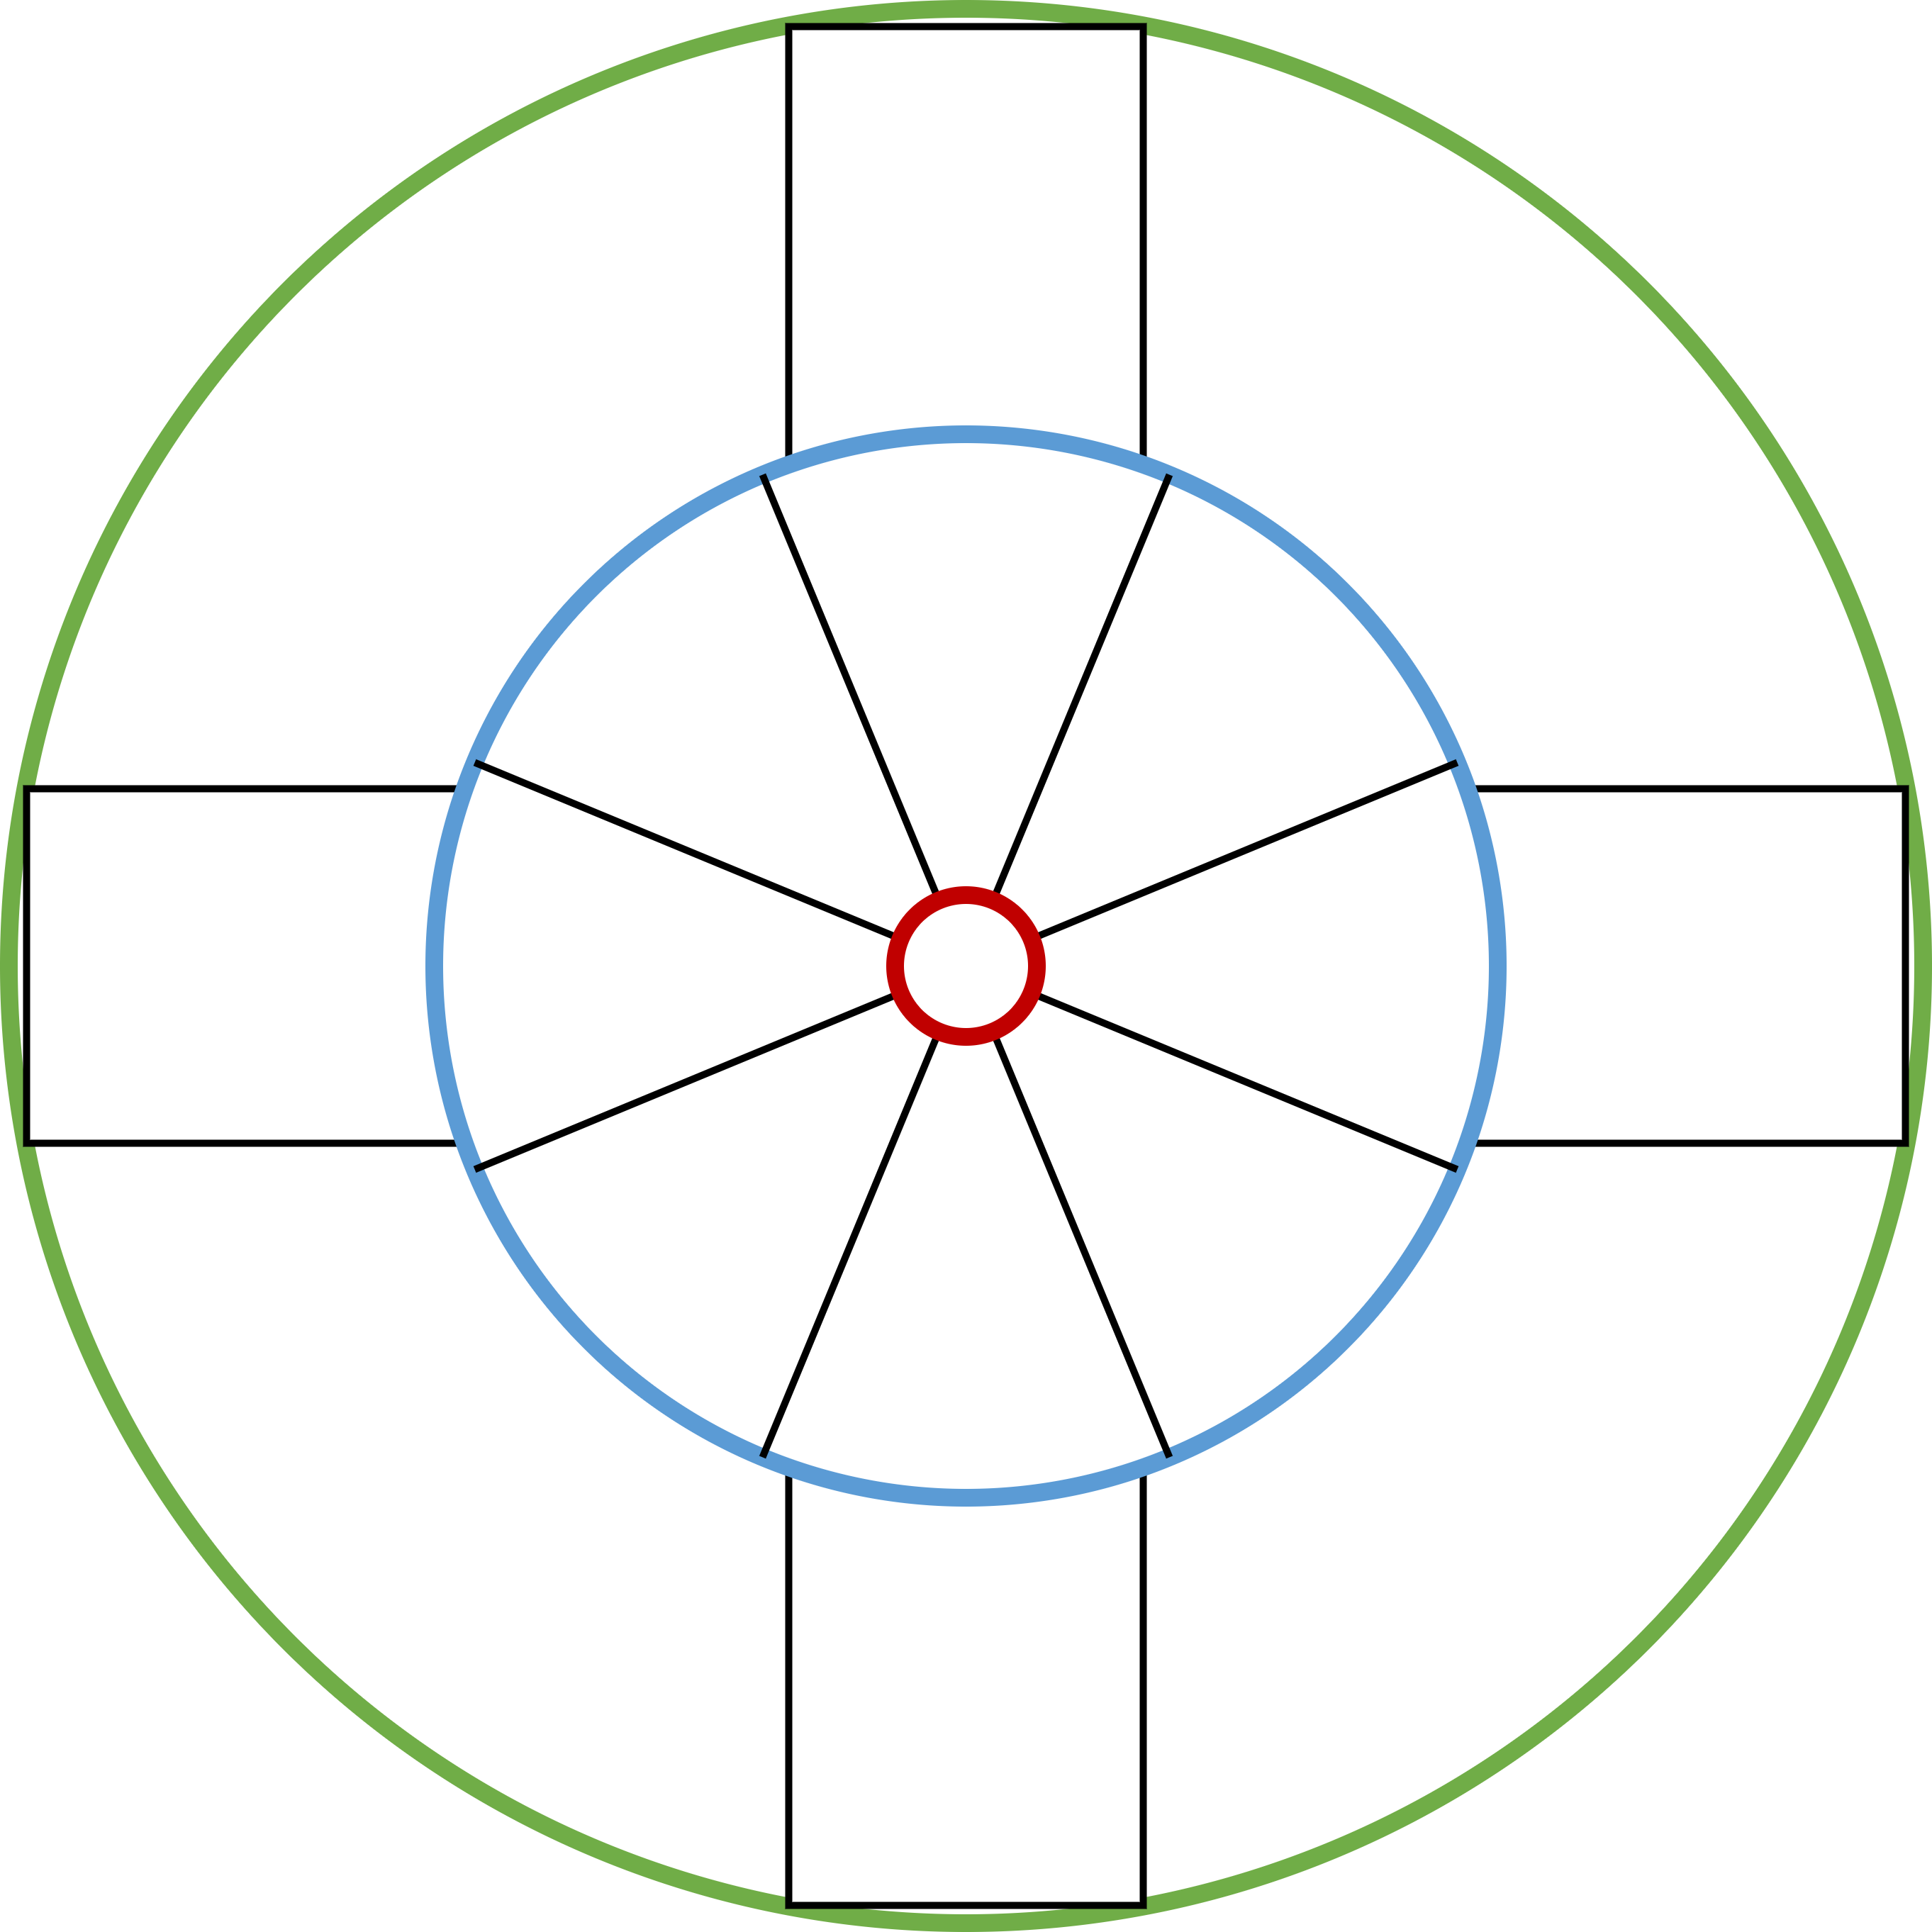
\includegraphics[width=0.3\textwidth]{images/konstruktionsgrößen.png}
  \caption{Konstruktionsgrößenanalyse}
  \label{fig:rondell_durchmesser}
\end{figure}

Umso kleiner dieser Durchmesser, je weniger Fahrräder können gelagert werden. Um den optimalen Wert zu finden, wurden Werte zwischen $0.1m-2.1m$ im Abstand von $0.1m$ getestet. Laut den Ergebnissen des Tests gibt es einen optimalen Wert, um die „Minimum“ Fläche (Blau) zu minimieren $d=1.4m$, um die „Maximum“ Fläche (Grün) zu minimieren, muss ein Durchmesser von über $2.2m$ gewählt werden.

\paragraph{Vorteile des Rondell Systems}
\begin{itemize}
  \item Gute Sichtbarkeit
  \item Hoher Wiedererkennungswert
  \item Optimales Einsatzgebiet in Parks und anderen nicht-rechteckigen Grundstücken.
  \item Einfache Erweiterbarkeit
  \item Fahrraddurchsatz je nach Anzahl der Lagerrobotern (Erweiterbar)
\end{itemize}

\paragraph{Nachteile des Rondell Systems}
\begin{itemize}
  \item Platzverschwendung durch pizzastückförmige Boxen. (Rechteckige Boxen passen besser auf die Form der Fahrräder)
  \item Es werden mehrere Lagerroboter benötigt (Je nach Konfiguration)
  \item Kompliziertes Lagersystem (Ein und Aushängen der Pizzastücke, Rotieren der gesamten Ebene)
  \item Neuartige Lagertechnologie, kann sich nicht auf bestehende Systeme Stützen
\end{itemize}
